%!TEX root = ./main.tex

\renewcommand{\inPoints}{}

\pgfmathsetmacro\pointsPerLine{4}% in [1,\infty[
\newsavebox\geometrya
\sbox{\geometrya}{%
	\pgfmathsetmacro\dimension{1}% in [0,3]
	%---------------------------------
% Auto config
\pgfmathsetmacro\xdim{\dimension>0}%
\pgfmathsetmacro\ydim{\dimension>1}%
\pgfmathsetmacro\zdim{\dimension>2}%
\pgfmathsetmacro\pointsPerLineMinusOne{\pointsPerLine-1}%
\pgfmathsetmacro\xnbr{\pointsPerLineMinusOne*\xdim}%
\pgfmathsetmacro\ynbr{\pointsPerLineMinusOne*\ydim}%
\pgfmathsetmacro\znbr{\pointsPerLineMinusOne*\zdim}%

%---------------------------------
% Figure
\begin{tikzpicture}[x={(1pt,0pt)},y={(0pt,1pt)},z={(0.45pt,0.35pt)}]
	\tikzset{point/.style={
		draw,
		circle,
		minimum size=\pointsize,
		inner sep=0,
	}}

	% Coordinates
	\foreach \x in {0,...,\xnbr}
	{
		\foreach \y in {0,...,\ynbr}
		{
			\foreach \z in {0,...,\znbr}
			{
				\pgfmathsetmacro\num{int(\x+(\pointsPerLine*\y)+(\pointsPerLine*\pointsPerLine*\z))}
				\coordinate (point\num) at (\pointssep*\x,\pointssep*\y,\pointssep*\z) {};
				\coordinate (point_\x_\y_\z) at (\pointssep*\x,\pointssep*\y,\pointssep*\z) {};
			}
		}
	}

	% Lines
	\foreach \x in {0,...,\xnbr}
	{
		\foreach \y in {0,...,\ynbr}
		{
			\foreach \z in {0,...,\znbr}
			{
				\ifthenelse{\x=0}{}{
					\pgfmathsetmacro\lastx{int(\x-1)}
					\draw[line width=\lineswidth,lines_color] (point_\lastx_\y_\z) -- (point_\x_\y_\z);
				}
				\ifthenelse{\y=0}{}{
					\pgfmathsetmacro\lasty{int(\y-1)}
					\draw[line width=\lineswidth,lines_color] (point_\x_\lasty_\z) -- (point_\x_\y_\z);
				}
				\ifthenelse{\z=0}{}{
					\pgfmathsetmacro\lastz{int(\z-1)}
					\draw[line width=\lineswidth,lines_color] (point_\x_\y_\lastz) -- (point_\x_\y_\z);
				}
			}
		}
	}

	% Points and numbers
	\foreach \x in {0,...,\xnbr}
	{
		\foreach \y in {0,...,\ynbr}
		{
			\foreach \z in {0,...,\znbr}
			{
				% Config
				\pgfmathsetmacro\num{int(\x+(\pointsPerLine*\y)+(\pointsPerLine*\pointsPerLine*\z))}
				\pgfmathsetmacro\pointsize{\pointssize*5/(5+\z+1)}

				% Draw point
				\node[
					point,
					points_boder_color,
					fill=points_color
				] at (point_\x_\y_\z.center) {};

				% Fill point if is in
				\foreach \i in \inPoints
				{
					\ifthenelse{\num=\i}{
						\node[
							point,
							points_boder_color,
							fill=in_points_color
						] at (point\i.center) {};
					}{}
				}

				% Number
				\pgfmathsetmacro\num{int(\x+(\pointsPerLine*\y)+(\pointsPerLine*\pointsPerLine*\z))}
				\node[below right=3pt] at (point_\x_\y_\z.center) {\small\num};
			}
		}
	}
\end{tikzpicture}
%
}
\newsavebox\geometryb
\sbox{\geometryb}{%
	\pgfmathsetmacro\dimension{2}% in [0,3]
	%---------------------------------
% Auto config
\pgfmathsetmacro\xdim{\dimension>0}%
\pgfmathsetmacro\ydim{\dimension>1}%
\pgfmathsetmacro\zdim{\dimension>2}%
\pgfmathsetmacro\pointsPerLineMinusOne{\pointsPerLine-1}%
\pgfmathsetmacro\xnbr{\pointsPerLineMinusOne*\xdim}%
\pgfmathsetmacro\ynbr{\pointsPerLineMinusOne*\ydim}%
\pgfmathsetmacro\znbr{\pointsPerLineMinusOne*\zdim}%

%---------------------------------
% Figure
\begin{tikzpicture}[x={(1pt,0pt)},y={(0pt,1pt)},z={(0.45pt,0.35pt)}]
	\tikzset{point/.style={
		draw,
		circle,
		minimum size=\pointsize,
		inner sep=0,
	}}

	% Coordinates
	\foreach \x in {0,...,\xnbr}
	{
		\foreach \y in {0,...,\ynbr}
		{
			\foreach \z in {0,...,\znbr}
			{
				\pgfmathsetmacro\num{int(\x+(\pointsPerLine*\y)+(\pointsPerLine*\pointsPerLine*\z))}
				\coordinate (point\num) at (\pointssep*\x,\pointssep*\y,\pointssep*\z) {};
				\coordinate (point_\x_\y_\z) at (\pointssep*\x,\pointssep*\y,\pointssep*\z) {};
			}
		}
	}

	% Lines
	\foreach \x in {0,...,\xnbr}
	{
		\foreach \y in {0,...,\ynbr}
		{
			\foreach \z in {0,...,\znbr}
			{
				\ifthenelse{\x=0}{}{
					\pgfmathsetmacro\lastx{int(\x-1)}
					\draw[line width=\lineswidth,lines_color] (point_\lastx_\y_\z) -- (point_\x_\y_\z);
				}
				\ifthenelse{\y=0}{}{
					\pgfmathsetmacro\lasty{int(\y-1)}
					\draw[line width=\lineswidth,lines_color] (point_\x_\lasty_\z) -- (point_\x_\y_\z);
				}
				\ifthenelse{\z=0}{}{
					\pgfmathsetmacro\lastz{int(\z-1)}
					\draw[line width=\lineswidth,lines_color] (point_\x_\y_\lastz) -- (point_\x_\y_\z);
				}
			}
		}
	}

	% Points and numbers
	\foreach \x in {0,...,\xnbr}
	{
		\foreach \y in {0,...,\ynbr}
		{
			\foreach \z in {0,...,\znbr}
			{
				% Config
				\pgfmathsetmacro\num{int(\x+(\pointsPerLine*\y)+(\pointsPerLine*\pointsPerLine*\z))}
				\pgfmathsetmacro\pointsize{\pointssize*5/(5+\z+1)}

				% Draw point
				\node[
					point,
					points_boder_color,
					fill=points_color
				] at (point_\x_\y_\z.center) {};

				% Fill point if is in
				\foreach \i in \inPoints
				{
					\ifthenelse{\num=\i}{
						\node[
							point,
							points_boder_color,
							fill=in_points_color
						] at (point\i.center) {};
					}{}
				}

				% Number
				\pgfmathsetmacro\num{int(\x+(\pointsPerLine*\y)+(\pointsPerLine*\pointsPerLine*\z))}
				\node[below right=3pt] at (point_\x_\y_\z.center) {\small\num};
			}
		}
	}
\end{tikzpicture}
%
}
\newsavebox\geometryc
\sbox{\geometryc}{%
	\pgfmathsetmacro\dimension{3}% in [0,3]
	%---------------------------------
% Auto config
\pgfmathsetmacro\xdim{\dimension>0}%
\pgfmathsetmacro\ydim{\dimension>1}%
\pgfmathsetmacro\zdim{\dimension>2}%
\pgfmathsetmacro\pointsPerLineMinusOne{\pointsPerLine-1}%
\pgfmathsetmacro\xnbr{\pointsPerLineMinusOne*\xdim}%
\pgfmathsetmacro\ynbr{\pointsPerLineMinusOne*\ydim}%
\pgfmathsetmacro\znbr{\pointsPerLineMinusOne*\zdim}%

%---------------------------------
% Figure
\begin{tikzpicture}[x={(1pt,0pt)},y={(0pt,1pt)},z={(0.45pt,0.35pt)}]
	\tikzset{point/.style={
		draw,
		circle,
		minimum size=\pointsize,
		inner sep=0,
	}}

	% Coordinates
	\foreach \x in {0,...,\xnbr}
	{
		\foreach \y in {0,...,\ynbr}
		{
			\foreach \z in {0,...,\znbr}
			{
				\pgfmathsetmacro\num{int(\x+(\pointsPerLine*\y)+(\pointsPerLine*\pointsPerLine*\z))}
				\coordinate (point\num) at (\pointssep*\x,\pointssep*\y,\pointssep*\z) {};
				\coordinate (point_\x_\y_\z) at (\pointssep*\x,\pointssep*\y,\pointssep*\z) {};
			}
		}
	}

	% Lines
	\foreach \x in {0,...,\xnbr}
	{
		\foreach \y in {0,...,\ynbr}
		{
			\foreach \z in {0,...,\znbr}
			{
				\ifthenelse{\x=0}{}{
					\pgfmathsetmacro\lastx{int(\x-1)}
					\draw[line width=\lineswidth,lines_color] (point_\lastx_\y_\z) -- (point_\x_\y_\z);
				}
				\ifthenelse{\y=0}{}{
					\pgfmathsetmacro\lasty{int(\y-1)}
					\draw[line width=\lineswidth,lines_color] (point_\x_\lasty_\z) -- (point_\x_\y_\z);
				}
				\ifthenelse{\z=0}{}{
					\pgfmathsetmacro\lastz{int(\z-1)}
					\draw[line width=\lineswidth,lines_color] (point_\x_\y_\lastz) -- (point_\x_\y_\z);
				}
			}
		}
	}

	% Points and numbers
	\foreach \x in {0,...,\xnbr}
	{
		\foreach \y in {0,...,\ynbr}
		{
			\foreach \z in {0,...,\znbr}
			{
				% Config
				\pgfmathsetmacro\num{int(\x+(\pointsPerLine*\y)+(\pointsPerLine*\pointsPerLine*\z))}
				\pgfmathsetmacro\pointsize{\pointssize*5/(5+\z+1)}

				% Draw point
				\node[
					point,
					points_boder_color,
					fill=points_color
				] at (point_\x_\y_\z.center) {};

				% Fill point if is in
				\foreach \i in \inPoints
				{
					\ifthenelse{\num=\i}{
						\node[
							point,
							points_boder_color,
							fill=in_points_color
						] at (point\i.center) {};
					}{}
				}

				% Number
				\pgfmathsetmacro\num{int(\x+(\pointsPerLine*\y)+(\pointsPerLine*\pointsPerLine*\z))}
				\node[below right=3pt] at (point_\x_\y_\z.center) {\small\num};
			}
		}
	}
\end{tikzpicture}
%
}

\begin{frame}
	\begin{minipage}{\textwidth}
		\centering%
		$S_k(3) = \underbrace{PG(1,3) \otimes \dots \otimes PG(1,3)}_{k\text{ times}}$
	\end{minipage}
	\resizebox{\textwidth}{!}{
		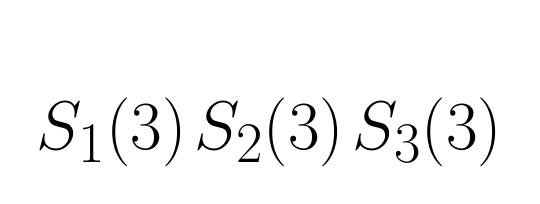
\begin{tikzpicture}
			\uncover<2->{
				\node (geometrya) at (0,0) {\usebox{\geometrya}};
				\node[anchor=north,yshift=-15,font=\Huge] at (geometrya.south) {$S_1(3)$};
			}
			\uncover<3->{
				\node[anchor=south west, xshift=50] (geometryb) at (geometrya.south east) {\usebox{\geometryb}};
				\node[anchor=north,yshift=-15,font=\Huge] at (geometryb.south) {$S_2(3)$};
			}
			\uncover<4->{
				\node[anchor=south west, xshift=50] (geometryc) at (geometryb.south east) {\usebox{\geometryc}};
				\node[anchor=north,yshift=-15,font=\Huge] at (geometryc.south) {$S_3(3)$};
			}
		\end{tikzpicture}
	}
	\begin{tikzpicture}[remember picture,overlay,x={(1pt,0pt)},y={(0pt,1pt)}]
		\node[anchor=south east] at ($(current page.south east)+(-3,10)$) {\tiny\textit{S stands for Segre varieties}};
	\end{tikzpicture}
\end{frame}
